% Author: Izaak Neutelings (February 2020)
% page 8 https://archive.org/details/StaticAndDynamicElectricity
% https://tex.stackexchange.com/questions/56353/extract-x-y-coordinate-of-an-arbitrary-point-on-curve-in-tikz
% https://tex.stackexchange.com/questions/412899/tikz-calculate-and-store-the-euclidian-distance-between-two-coordinates

\documentclass[border=3pt,tikz]{standalone}
\usepackage{amsmath} % for \dfrac
\usepackage{physics}
\usepackage{tikz,pgfplots}
\usetikzlibrary{angles,quotes} % for pic (angle labels)
\usetikzlibrary{decorations.markings}
\tikzset{>=latex} % for LaTeX arrow head

\usepackage{xcolor}
\colorlet{Ecol}{orange!90!black}
\colorlet{Vcol}{blue!90!black}
\colorlet{veccol}{green!45!black}
\tikzstyle{EField}=[thick,Ecol]
\tikzstyle{VField}=[thick,Vcol]
\def\tick#1#2{\draw[thick] (#1) ++ (#2:0.03*\ymax) --++ (#2-180:0.06*\ymax)}


\begin{document}


% ELECTRIC FIELD of a CHARGED SPHERE
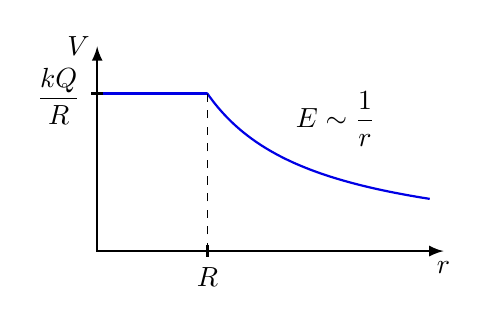
\begin{tikzpicture}
  \def\xmax{4.4}
  \def\ymax{2.6}
  \def\kQ{2.8}
  \def\R{1.4}
  \coordinate (O) at (0,0);
  \coordinate (X) at (\xmax,0);
  \coordinate (Y) at (0,\ymax);
  \coordinate (P) at (\R,\kQ/\R);
  \coordinate (Px) at (\R,0);
  \coordinate (Py) at (0,\kQ/\R);
  
  % PLOT
  \draw[VField,samples=100,smooth,variable=\x,domain=\R:0.96*\xmax]
    (Py) -- plot(\x,\kQ/\x);
  \draw[VField]
    (Py) --++ (Px);
  \node[above right] at (2.4,1.2) {$E \sim \dfrac{1}{r}$};
  \draw[dashed]
    (Px) -- (P);
  
  % AXIS
  \draw[<->,thick]
    (X) node[below] {$r$} -- (O) -- (Y) node[left=-1] {$V$};
  \tick{Py}{ 0} node[below=1,left] {$\dfrac{kQ}{R}$};
  \tick{Px}{90} node[below] {$R$};
  
\end{tikzpicture}


\end{document}
